% !TEX root=/home/tavant/these/manuscript/src/manuscript.tex

\section{Bidimensional simulation of an \ac{HET}}

We are interested in studying the azimuthal instabilities and the induced electron transport in the axial direction.
In addition, we want to study the plasma-wall interactions.
As realistic \ac{3D} simulations are not yet achievable, we choose to simulate the radial-azimuthal plane.
The axial location where the electron drift is the highest is close to the exit plane, where the axial electric field is the highest.
Hence, we choose this location to be simulated.
In this section, we describe the characteristics of the radial-azimuthal simulation.


\subsection{Neglecting curvature}
The \ac{ECDI} features oscillations of short wavelength of the order of the mm.
Hence, neglecting the curvature of the channel is expected not to change the \ac{ECDI} characteristics while improving the simulation performances.

In  \citet{heron2013},  the authors have performed a \ac{2D} \ac{PIC} simulation including the channel curvature.
They have observed a small difference between the inner and the outer walls.
In  \citet{dominguez-vazquez2018}, the authors studied the effect of the curvature using a \ac{1D} radial model.
They have shown asymmetries due to the combination of the geometric expansion, the magnetic mirror effect, and the centrifugal force.
However, the global behavior of the discharge is not affected compared to simulations without the curvature model.
Hence, in order to simplify the analogy, we choose to neglect the curvature.

Consequently, we can use a Cartesian mesh (also called a rectangular mesh).
The usual notation $x,y$ is used in the simulation for the radial ($r$) and azimuthal directions $\theta$, respectively.
The $z$ component corresponds to the axial direction, normal to the simulation domain.

\subsection{Radial-azimuthal domain description}

The azimuthal direction is closed using a periodic boundary condition for both the particles and the fields.
Consequently, when a particle crosses the azimuthal boundary, it is moved to the other side of the domain.
The plasma potential and the azimuthal electric field are continuous in the azimuthal direction.
The radial direction is closed by the walls.
They can be grounded metallic, or a dielectric boundary can be modeled.
The physics related to the boundary conditions of the walls are described and discussed in \cref{sec-diel}.

A constant and uniform magnetic field $B_0$ is imposed in the radial direction.
This does not take into account the magnetic mirror, that has been shown to be important \citep{keidar2005,yu2008a,dominguez-vazquez2018}.
However, it cannot be modeled in the \ac{2D} Cartesian radial-azimuthal domain while conserving a divergent-free magnetic field topology.
A constant and uniform axial electric field $E_0$ is imposed.
\Cref{fig-2dschemat} shows a schematic representation of the simulated domain, overlaid with the computed azimuthal electric field $E_y$.

\begin{figure}[hbtp]
  \centering
  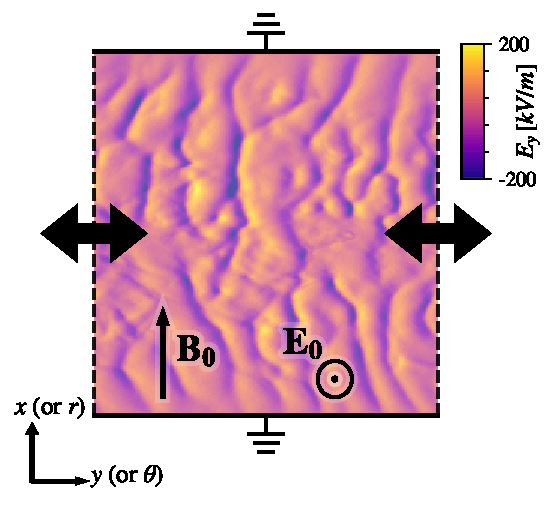
\includegraphics[width=\defaultwidth]{2D_schema.pdf}
  \caption{Schematic representation of the radial-azimuthal simulation domain. Overlaid is the computed azimuthal electric field given as an example. The radial length is 2\,cm, and the azimuthal length is 1\,cm.
  The magnetic field is $B_0=0.02\,\tesla$, the axial electric field is $E_0=\sn{2}{4}\,\volt\per\meter$, and the walls are grounded. More parameters are given in \cref{parameters}.}
  \label{fig-2dschemat}
\end{figure}

\subsection{Particle balance}
As the axial position simulated is the exit plane, the ionization is too low to balance the particle losses to the wall.
Instead, the ionization takes place upstream, and the particles are convected downstream.
In these conditions, two models can be used concerning the particle losses at the walls\string:
\begin{itemize}
  \item having a simulation that dies off, as done in \citet{janhunen2018},
  \item forcing an arbitrary ionization to occur in order to compensate the radial losses \citep{dominguez-vazquez2018}.
\end{itemize}
The second option is slightly less realistic, but allows to obtain a steady-state and is supposed not to affect the simulation significantly.
Hence, we use this model to achieve a constant mean plasma density during the simulation.
The forced ionization rate is computed in order to compensate the losses of the ions at each time step.
The spatial ionization  profile is uniform.


\subsection{Axial convection}

Due to the imposed axial electric field, ions and electrons gain energy.
In the \ac{HET}, the axial convection of the particles balances the energy gain.
However, in a purely \ac{2D} simulations, the convection is missing, resulting in an ever-rising particle energy.
This prevents the possibility to reach a steady-state regime, as observed in \citet{heron2013,janhunen2018}.

We implemented a model of convection initially proposed for a \ac{1D} simulation by \citet{lafleur2016a}, and adapted in \ac{2D} by \citet{croes2017a}.
The model uses a finite axial length $L_z$.
When a particle reaches the boundary $z=0$ or $z=L_z$, it is removed from the simulation.
In order to conserve the particle (and charge) balance, a particle is created at $z=0$ for the ions (that are accelerated toward $z>0$) or at $z=L_z$ for the electrons.
It has been observed that using a radial position chosen uniformly at random for the newly injected particle would affect the sheath \citep{croes2017a}.
Hence, the radial position of the new particle is the same as the removed particle.

Concerning the azimuthal particle position, it is more difficult to choose between a random position or the same position as the removed particle.
In \citet{lafleur2016a,croes2017a}, a random azimuthal position was chosen.
However, as will be discussed in \cref{sec-reinjectionnoise}, this induces a numerical noise that can be harmful in some cases.
